\section{Results}\label{sec:results}
\subsection{Sharpness and numerical reliability}
Validation of the population solver covers 280 instances, being 14 laws applied to each of the 4 partition divisions and 5 offsets in information level. In every instance, results match the standalone oracle. Maximum difference in upper risk (in absolute value) was less than $4.615\times10^{-13}$, or $4.002\times10^{-13}$ for the 360 profiles considered in the decisions experiment. These are sanity checks on our evaluation of solution limits, while tightness is demonstrated directly from Theorem~\ref{thm:sharp}. Cases where no limit can be ascertained are dealt with in both the existing oracle and proof of the theorem (not derived from the match across the remaining 280 instances).

All 54 tests checking for consistent partitions across different partition levels exhibit the expected nested structure, and 18 cases checking earlier and 24 checking matching termination points met the corresponding test criterion. Checks on splitting of the profile, concavity, minimum attainable compatibility and completions were also recorded and align with theory. Additionally, we observed 33/40 cases for which there is an envelope that can be compared with an oracle-computed feasible risk, and no case where our upper-risk value fell below this oracle quantity. 7 cases did not have a feasible risk from the oracle to compare against. Across these instances, we confirm matching solution between restricted decisions and unrestricted search over 176 resource-allocation decisions. This does not constitute an exhaustive test over all runs and roundings, but demonstrates that the desired property holds for our decision-search procedure.
\subsection{Timing changes population certification decisions}
Table~\ref{tab:population} gives a common-budget comparison for the timing-and-terminal harmful-late law. At $\rho=0.05$, every displayed partition is compatible. Endpoint information gives an upper risk of $0.065835$, exceeding $\beta=0.06$. Two bands suffice to cross the decision threshold, and further refinement lowers the upper endpoint to $0.055241$ at eight bands. The observed outcome and terminal-selection marginals are identical across these analyses.

\begin{table}[!htbp]\centering
\caption{Population decision value at $\rho=0.05$ and $\beta=0.06$ for the timing-and-terminal harmful-late law. Information quantities are in nats. A decision is a sharp population statement, without sampling uncertainty.}\label{tab:population}
\begin{tabular}{rrrrl}\toprule $K$ & $\tau_K$ & $\theta_{U,K}(0.05)$ & $\rho_K^*(0.06)$ & Decision\\\midrule
1 & 0.000000 & 0.065835 & 0.035491 & Uncertified\\
2 & 0.018323 & 0.058346 & 0.053814 & Certified\\
4 & 0.023710 & 0.055899 & 0.059201 & Certified\\
8 & 0.025106 & 0.055241 & 0.060597 & Certified\\\bottomrule\end{tabular}

\end{table}

Complete-case risk here is $\td = 0.037333$, with assumption-free bound $A+c = 0.0975$ and 8-band lower limit of 0.025106. Introducing time shifts the certified region along $\beta = 0.06$ from 0.035491 (endpoint) to 0.060597 (8-band). In other words, we have increased the certified value for $\rho$ over an interval of width 0.025106 nats (= size of timing improvement), i.e. $(0.035491,0.060597]$, which is above the corresponding 8-band compatibility limit. The relationship between the sensitivity and profile bounds is summarised in Figure~\ref{fig:identification}.

One may similarly consider the fraction of failures that could remain among incompletely-observed outcomes under a given allowed sensitivity. Under the target population rule, Table~\ref{tab: population}, this ratio is $A/r=0.0373$ amongst completed observations. The implied tolerable fractions of failures if incompletes occur, at $\rho=0.05$, are ~0.493 for the endpoint bound and 0.324 for 8-band timing. These amounts to odds ratios of approximately 25.1 / 12.4 against the fraction of known failures, again purely bounding the possible extent of failure given the choice of maximum tolerance.

Overall we find 34/2160 rules where decisions switch from no-certification (endpoint) to some degree of certification with timing: 13, 11, 10 under the timing & terminal, high-incomplete and timing-only selection criteria respectively. Obviously these are numbers of scenarios considered rather than any statement about expected utility gains in a trial. None of the auxiliary control choices (no path dependence; terminal only; low failure rate) altered decisions on this range. The unremarkably tight margin by which the standard harmful-late choice is certified at $\rho=0.05$ (8 band), $\beta=0.06$, is mirrored by a null result when assessed by its intrinsic confirmatory power: <1% of 100 MC experiments reach the 20k sample limit at either endpoint or 8-band timing. We will examine the corresponding sample-size performance for a different, higher-power timing regime subsequently.
\subsection{Finite-sample certification under informative timing}
The strong-timing law has a true risk of $0.02$. For $\rho=0.08$, the population sharp upper risks for $K=1,2,4,8$ bands are $0.079617$, $0.059129$, $0.049755$ and $0.047196$. With $\beta=0.09$, all $K$-band procedures are certifiable, though with widely different slack and (for fixed number of observations) degrees of freedom.

Figure~\ref{fig:power}(a) and Table~\ref{tab:power} illustrate these certification probabilities. With $K=2$, all 100 streams are certifiable at 5,000 matured events (probability lower bound $[0.964, 1]$). For $K=1$ (i.e. using stream endpoints only), there are no certifications before 5,000 events and 96 of 100 are certified at 50,000 matured events (probability lower bound $[0.901, 0.989]$). Of course, 5,000 matured events represents one tenth of the matured events considered for $K=1$. This example does not imply that $K=1$ requires ten times as many observations to achieve any level of probability of certification. Certifications for $K=4$ occur at 88/100 streams after 5,000 matured events and 100/100 at 10,000 matured events, while $K=8$ shows 98/100 streams after 10,000 matured events. Hence more finely-resolved timing allows certification at earlier stages, although less finely-resolved timing yields the lowest upper bound on the population risk.

Incomplete numerical optimisation contributes to this discrepancy but cannot entirely account for it: the decision-targeted searches show that 89 of the 96 streams certified at 50,000 events would not have been certifiable after only 5,000 events (and 7 were numerically inconclusive). By contrast, using two bands per stream resulted in every stream being certifiable after 5,000 matured events. At longer timescales, failures to resolve the numerical search completely will additionally reduce the number of certifiable streams. The four streams from the exhaustive search case are omitted from the preceding calculation and remain in the 'full search' counts.

\begin{figure}[!htbp]
\centering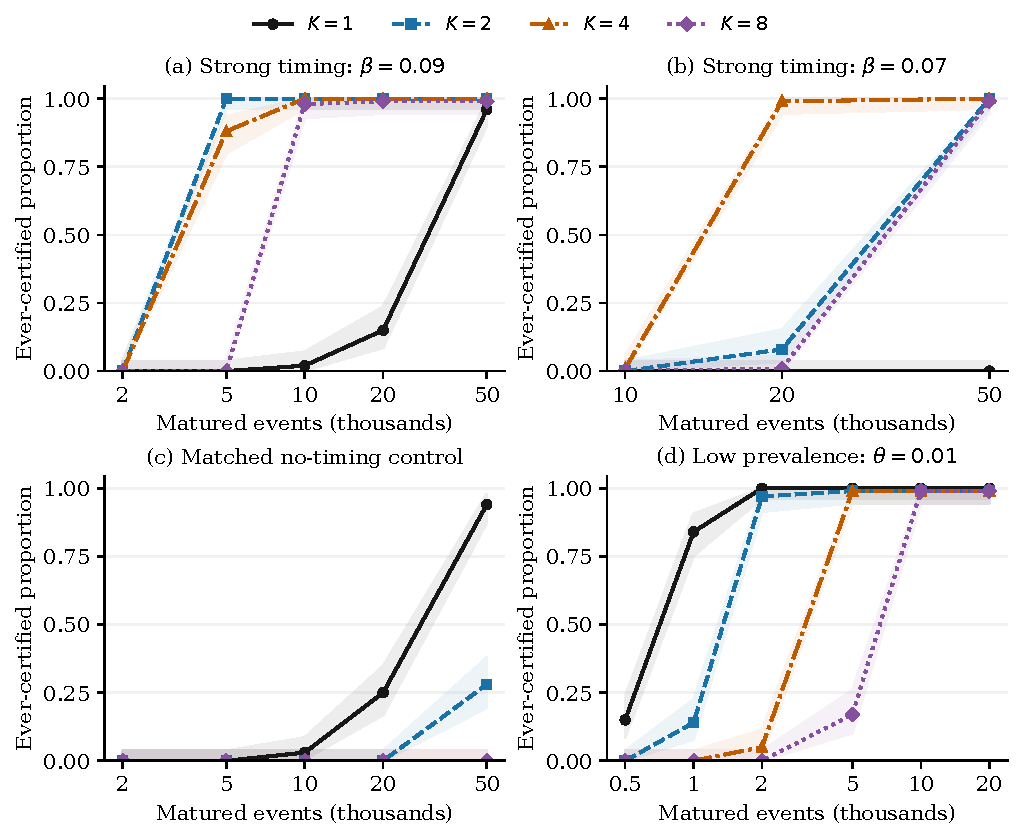
\includegraphics[width=\linewidth]{figures/certification_power.pdf}
\caption{Confirmatory certification by checkpoint, using 100 independent streams per scenario--partition cell and $\delta=0.05$ per fixed partition. Lines join observed ever-certified proportions; shaded bands are conditionwise exact two-sided 95\% Clopper--Pearson intervals. (a) Strong timing, $\rho=0.08,\beta=0.09$. (b) The same law and $\rho$, with $\beta=0.07$, below the endpoint population upper bound. (c) Matched endpoint masses with no timing contrast, $\rho=0.08,\beta=0.09$. (d) Low-prevalence law, $\rho=0.02,\beta=0.05$. Partition analyses within a law share finest-resolution streams. Checkpoints within a stream are dependent.}\label{fig:power}
\end{figure}

\begin{table}[!htbp]\centering
\caption{Selected strong-timing certification results at $\rho=0.08$. Counts refer to ever certifying by the stated horizon. Intervals quantify Monte Carlo certification probability across 100 streams, separately for each row. The full checkpoint curves and matched control are in Figure~\ref{fig:power}.}\label{tab:power}
\begin{tabular}{rrrrl}\toprule $\beta$ & $K$ & Horizon $n$ & Certified streams & Exact 95\% interval\\\midrule
0.09 & 1 & 50,000 & 96/100 & [0.9007, 0.9890]\\
0.09 & 2 & 5,000 & 100/100 & [0.9638, 1.0000]\\
0.09 & 4 & 5,000 & 88/100 & [0.7998, 0.9364]\\
0.09 & 4 & 10,000 & 100/100 & [0.9638, 1.0000]\\
0.09 & 8 & 10,000 & 98/100 & [0.9296, 0.9976]\\
0.07 & 1 & 50,000 & 0/100 & [0.0000, 0.0362]\\
0.07 & 2 & 50,000 & 100/100 & [0.9638, 1.0000]\\
0.07 & 4 & 20,000 & 99/100 & [0.9455, 0.9997]\\
0.07 & 8 & 50,000 & 99/100 & [0.9455, 0.9997]\\\bottomrule\end{tabular}

\end{table}
\FloatBarrier

For the tighter threshold of $\beta=0.07$, the endpoint is certifiable in population although the minimum upper end of its identified set is greater than $\beta$. All partition schemes are again certifiable in population: with endpoint one can certify 0 out of 100 trajectories given 50,000 observations, $K=2$ allows 100/100 certification within 50,000, $K=4$ achieves 99/100 certification within 20,000 and all 100 within 50,000, and $K=8$ achieves 99/100 within 50,000. Hence, using trajectory refinement changes whether trajectories can be certified in population as well as the empirical rate at which this occurs. Non-certifiability of the endpoint in population merely reflects the extent of the endpoint's identified set, and would only prevent (simultaneous) trajectory-wise certification if it occurred outside of the containment probability.

We additionally examine non-vacuity in the context of lower prevalence, i.e. with $\theta=0.01,\rho=0.02,\beta=0.05$. The endpoint yields 100/100 certification within 2000 observations, versus 2/4/8 partitioned trajectories at 97/99/99 certification levels respectively by 2000/5000/10000 observations. This is expected since the endpoint's margin for error is large and hence more finely-partitioned intervals need not substantially shorten the required observation times to achieve the corresponding certification rates.

\subsection{When resolution pays for its statistical cost}
As before, the mass assigned to each endpoint matches that of the strong-timing law. There are no timing observations available for this no-timing counterpart. Population maximum bounds are identical ($0.079617$) across all 4 partitions. Certified streams drop rapidly from 94/100 to 0/100 over $K=1,...,8$ for 50,000 events (Fig.~\ref{fig: power}c), as expected when increasing partition size while retaining only non-informative timing data. We interpret this loss in power to be attributable to finite sample variation in the categorical marginals, looser envelopes based on aggregated timing, and/or search incompleteness. Two-band target-oriented searches were completed by 50k events with 27 certified + 1 refuted + 67 ongoing + 1 halted (out of 96 streams); 8-band target-oriented with 94 refuted + 2 halted (out of 96). The 4 complete search cases are subsumed within the corresponding 100-stream numbers reported above (see Supp.). Theorem~\ref{thm: refinement} only applies to comparing population-level identifiability between varying K, and not to envelope coverage of individual samples.

We also note additional considerations arising from the supplementary comparisons against these procedures. Certifications by the repeated-static (i.e. time-nonuniform) monitoring at $n = 500$ are 71/100 (vs. 15/100 for TrajCert) and at $n = 1000$, 99/100 (vs. 84/100). This gain in power naturally occurs at the expense of losing time-uniformity. Dense-monitoring comparisons were unable to certify under the pre-specified FWER limit and we therefore cannot claim optional-stopping error under repeated-static monitoring in that context. The procedure from \cite{...}, under the assumptions of ignorable delay (i.e. no sensitivity to the underlying delay process required), can certify by 20k events at 98/100 streams; ours at $K=1$ yields 98/100 but decreases to 0/100 by $K=8$. It should again be expected given its more stringent identifiability setup. Remaining comparison scenarios yielding no certifications are presented in the Supp.

\subsection{Time-uniform validity diagnostics}
Table~\ref{tab:coverage} summarizes the seven retained validity scenarios. TrajCert's recorded violation diagnostic counts either an empty running region or a reported risk upper bound below the known risk. Its counts agree with the categorical-construction counts in these artifacts: one stream in the independent-resolution control, one in high unresolvedness, and none in the other five scenarios. Both nonzero diagnostics arise from empty running regions. The exact one-sided upper limits are $0.00945$ for 1/500 and $0.00597$ for 0/500, both below the configured 0.06 acceptance limit. All seven cells complete without technical failure. These conditionwise checks are consistent with the theorem but neither prove it nor establish a simultaneous 95\% campaign-level coverage statement. No scenario certifies within 500 events; certification power is evaluated separately above.

\begin{table}[!htbp]\centering
\caption{Time-uniform validity diagnostics through 500 matured events per stream, with risk projections at 100-event checkpoints. Each scenario has 500 independent streams. Limits are exact one-sided 95\% limits for the recorded ever-violation event, separately by scenario. The configured acceptance limit is 0.06, while the nominal theoretical level is $\delta=0.05$.}\label{tab:coverage}
\begin{tabular}{lrrr}\toprule Scenario & $K$ & Violations / streams & One-sided 95\% upper\\\midrule
High unresolvedness & 8 & 1/500 & 0.00945\\
Independent resolution & 8 & 1/500 & 0.00945\\
Low prevalence & 8 & 0/500 & 0.00597\\
Minimum-information completion & 8 & 0/500 & 0.00597\\
Near certification boundary & 8 & 0/500 & 0.00597\\
Near degeneracy & 8 & 0/500 & 0.00597\\
Thirty-two bands & 32 & 0/500 & 0.00597\\\bottomrule\end{tabular}

\end{table}

There are no false risk certificates among the 32 power cells (0/100, corresponding to a 95% one-sided upper bound of $0.02951$ for each cell). Likewise, no certificates are issued in cells that have a compatible data-generating process and known upper risk exceeding $\beta$. We emphasise this need not imply that the chance of error is zero; e.g. the number of sequences excluding the true data generating process varies from 1 to 6 out of 100 in each cell, reflecting the fact that the result holds with high rather than sure probability. In one cell we specify an incompatible budget ($K=4$), and observe that 16/100 sequences issue a certificate by t=20000. Again, these do not constitute false risk certificates because the true risk is < $\beta$. None of the tested times indicate an incompatible data generating process, including the two incompatible-budget cells; i.e. the incompatibility test fails to flag an incompatible budget at these sample sizes. There is thus no evidence to infer the declared sensitivity constraint, and we omit these cells from inferences made assuming a valid data generating process. Full details are given in the Supplement. 

\subsection{Computation and sensitivity boundaries}
Figure~\ref{fig:computation} separates the two computational scales. Population median runtimes are $0.334$--$0.403$ ms over $K=1$--128, with a reported median of 36 total root iterations at every $K$. Oracle discrepancies in this benchmark do not exceed $3.592\times10^{-13}$. The broader 500-event outer-projection target takes median $0.809$--$6.044$ seconds, with peak process resident memory $215.35$--$226.89$ MiB. These process-memory measurements include the Python runtime and libraries. Finite-sample projection is substantially more expensive than the scalar population solve; a conservative early return can also be less tight than the optimization target. Neither the runtime benchmark nor a node cap establishes a worst-case complexity bound for the projection.

The power-study checkpoints also serve to quantify an extra computational cost. We obtained 160 run-time medians (one for each checkpoint), with overall median = 0.0725 s and maximum of 14.300 s, of which 7 had values over 10 s. These results are based on the other three search representatives for each cell (excluding the 4 full-search runs), i.e. they measure the additional runtime of running the projections for the checkpoints. Note that these should not be interpreted in relation to our standalone timing study of runtime-scaling. The existing machine information does not allow a generalised statement on run-time.

\begin{figure}[!htbp]
\centering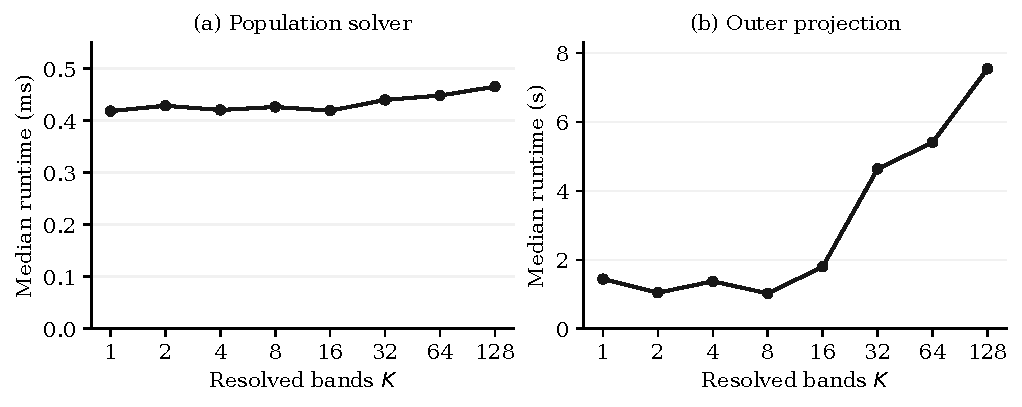
\includegraphics[width=\linewidth]{figures/computation.pdf}
\caption{Computational benchmark from existing records: medians of 30 isolated measured invocations after five warmups per $K$, with numerical-library threads limited to one. (a) Population solver, including law and summary construction. (b) Broader outer target, including a deterministic 500-event ledger, sequential confidence updates and the final projection. The law form is regenerated at each $K$, and both targets use its true information plus 0.01 nats. These curves measure cost, not nested-law information gain.}\label{fig:computation}
\end{figure}
\FloatBarrier

No separate estimator is needed to characterise the different sensitivity regimes - this is provided by the compatible/risk bounds. For any given set of empirical margins, the length of the compatible (risk) interval increases with $\rho$; alternatively, refining the margins may lead to shrinkage of the compatible interval, or incompatibility, as a function of $\rho$. As an example, consider expected counts under the rare-disease scenario for $\rho=0.02, \beta = 0.05$, where the compatible intervals are bounded by 0.0540 and 0.0404 respectively, corresponding to sample sizes of 5k and 10k. This highlights the change of behaviour between these two sample sizes (again purely based on expected counts).

\FloatBarrier
